\newcommand{\base}{\ensuremath{\mathsf{base}}\xspace}
\newcommand{\lloop}{\ensuremath{\mathsf{loop}}\xspace}
\newcommand{\seg}{\ensuremath{\mathsf{seg}}\xspace}
\newcommand{\eqtopath}{\ensuremath{\mathsf{eqtopath}}\xspace}
\newcommand{\dpath}[4]{#3 =^{#1}_{#2} #4}

\chapter{Higher inductive types}
\label{cha:hits}

\section{Introduction to HITs}
\label{sec:intro-hits}

Like the general inductive types we discussed in Chapter~\ref{cha:induction}, \emph{higher inductive types} are a general schema for defining new types generated by some constructors.
But unlike ordinary inductive types, in defining a higher inductive type we may have ``constructors'' which generate not only \emph{points} of that type, but also \emph{paths} and higher paths in that type.
For instance, we can consider the higher inductive type $\Sn^1$ generated by
\begin{itemize}
\item A point $\base:\Sn^1$, and
\item A path $\lloop : {\id[\Sn^1]\base\base}$.
\end{itemize}
This should be regarded as entirely analogous to the definition of, for instance, $\bool$, as being generated by
\begin{itemize}
\item A point $0:\bool$ and
\item A point $1:\bool$,
\end{itemize}
or the definition of $\nat$ as generated by
\begin{itemize}
\item A point $0:\nat$ and
\item A function $s:\nat\to\nat$.
\end{itemize}
When we think of types as higher groupoids, the more general notion of ``generation'' is very natural:
since a higher groupoid is a ``multi-sorted object'' with paths and higher paths as well as points, we should allow ``generators'' in all dimensions.
However, there are some important points to be made regarding this generalization.

First of all, the word ``generation'' should be taken seriously, in the same sense that a group can be freely generated by some set.
In particular, because a higher groupoid comes with \emph{operations} on paths and higher paths, when such an object is ``generated'' by certain constructors, the operations will create more paths that don't come directly from the constructors themselves.
For instance, in the higher inductive type $\Sn^1$, the constructor $\lloop$ is not the only nontrivial path from $\base$ to $\base$; we have also $\lloop\ct\lloop$ and $\lloop\ct\lloop\ct\lloop$ and so on, as well as $\opp{\lloop}$, etc., all of which are different.
This may seem so obvious as to be not worth mentioning, but it is a departure from the behavior of ``ordinary'' inductive types, where one can expect to see nothing in the inductive type except what was ``put in'' directly by the constructors.

Secondly, this generation is really \emph{free} generation: higher inductive types do not technically allow us to impose ``axioms'', such as forcing $\lloop\ct\lloop$ to equal $\refl{\base}$.
However, in the world of $\infty$-groupoids, there is little difference between ``free generation'' and ``presentation'', since we can make two paths equal \emph{up to homotopy} by adding a new 2-dimensional generator relating them (e.g.\ a path $\lloop\ct\lloop = \refl{\base}$ in $\base=\base$).
We do then, of course, have to worry about whether this new generator should satisfy its own ``axioms'', and so on, but in principle any ``presentation'' can be transformed into a ``free'' one by making axioms into constructors.
As we will see, by adding ``truncation constructors'' we can use higher inductive types to express classical notions such as group presentations as well.

Thirdly, even though a higher inductive type contains ``constructors'' which generate \emph{paths in} that type, it is still an inductive definition of a \emph{single} type.
In particular, as we will see, it is the higher inductive type itself which will be given a universal property (expressed, as usual, by an induction principle), and \emph{not} its identity types.
The identity type of a higher inductive type retains the usual induction principle of any identity type (i.e.\ path induction), and does not acquire any new induction principle.

This implies that in general, it may be quite nontrivial to identify the identity types of a higher inductive type in any concrete way, in contrast to how in Chapter~\ref{cha:basics} we were able to give explicit descriptions of the behavior of identity types under all the traditional type forming operations.
For instance, are there any paths from $\base$ to $\base$ in $\Sn^1$ which are not simply composites of copies of $\lloop$ and its inverse?
Intuitively, it seems that the answer should be no (and it is), but proving this is not entirely trivial.
Indeed, such questions bring us rapidly to problems such as calculating the homotopy groups of spheres, a long-standing problem in algebraic topology for which no simple formula is known.
Homotopy type theory brings a new and powerful viewpoint to bear on such questions, but it also requires type theory to become as complex as the answers to these questions.

Fourthly, the ``dimension'' of the constructors (i.e.\ whether they output points, paths, paths between paths, etc.)\ does not have a direct connection to which dimensions the resulting type has nontrivial homotopy in.
As a simple example, if an inductive type $B$ has a constructor of type $A\to B$, then any paths and higher paths in $A$ will result in paths and higher paths in $B$, even though the constructor is not a ``higher'' constructor at all.
The same thing happens with higher constructors too: having a constructor of type $A\to (\id[B]xy)$ means not only that points of $A$ yield paths from $x$ to $y$ in $B$, but that paths in $A$ yield paths between these paths, and so on.
As we will see, this possibility is responsible for much of the power of higher inductive types.

On the other hand, it is even possible for constructors \emph{without} higher types in their inputs to generate ``unexpected'' higher paths.
For instance, in the 2-dimensional sphere $\Sn^2$ generated by
\begin{itemize}
\item A point $\base:\Sn^2$, and
\item A 2-dimensional path $\mathsf{surf}:\refl{\base} = \refl{\base}$ in ${\base=\base}$,
\end{itemize}
there is a nontrivial \emph{3-dimensional path} from $\refl{\refl{\base}}$ to itself.
Topologists will recognize this path as an incarnation of the \emph{Hopf fibration}.
From a category-theoretic point of view, this is the same sort of phenomenon as the fact mentioned above that $\Sn^1$ contains not only $\lloop$ but also $\lloop\ct\lloop$ and so on: it's just that in a \emph{higher} groupoid, there are \emph{operations} which raise dimension.
Indeed, we saw many of these operations back in \S\ref{sec:equality}: the associativity and unit laws are not just axioms but operations, whose inputs are 1-paths and whose outputs are 2-paths.


\section{Induction principles and dependent paths}
\label{sec:dependent-paths}

When we describe a higher inductive type such as the circle as being generated by certain constructors, we have to explain what this means by giving rules analogous to those for the basic type constructors from Chapter~\ref{cha:typetheory}.
The constructors themselves give the \emph{introduction} rules, but it requires a bit more thought to explain the \emph{elimination} rules.
In this book we will not attempt to give a general formulation of what constitutes a ``higher inductive definition'' and how to extract the elimination rule from such a definition --- indeed, this is a subtle question and the subject of current research.
Instead we will rely on some general informal discussion and numerous examples.

The non-dependent form of the eliminator is usually easy to describe: given any type equipped with the same structure with which the constructors equip the HIT in question, there is a function which maps the constructors to that structure.
For instance, in the case of $\Sn^1$, the non-dependent eliminator says that given any type $B$ equipped with a point $b:B$ and a path $\ell:b=b$, there is a function $f:\Sn^1\to B$ such that $f(\base)=b$ and $\ap f \lloop = \ell$ (the computation rules).

There is, however, a question of whether these computation rules are judgmental equalities or paths.
For ordinary inductive types, we had no qualms about making them judgmental; in that case one may argue that they are really \emph{definitional} equalities in the intuitive sense.
For higher inductive types, this is less clear, and it is likewise less clear to what extent these equalities can be made judgmental in the known set-theoretic models.
Moreover, since the operation $\apfunc f$ is not really a fundamental part of the type theory, but something that we \emph{defined} using the induction principle of identity types (and which we might have defined in some other, propositionally equal, way), it seems odd to refer to it explicitly in a judgmental equality.

There is generally consensus that the computational equalities for \emph{point} constructors, at least, should be judgmental.
In the example above, this means we have $f(\base)\jdeq b$.
This is unproblematic both philosophically and semantically.
Moreover, it greatly simplifies our lives, since otherwise the second computation rule $\ap f \lloop = \ell$ would not even be well-typed as a propositional equality; we would have to compose one side or the other with the specified identification of $f(\base)$ with $b$.
(Such problems do arise eventually, of course, when we come to talk about paths of higher dimension, but that will not be of great concern to us here.)
Thus, we will take the point-constructor computation rules to be judgmental, and those for paths and higher paths to be propositional.

Now, what about the dependent eliminator (the induction principle)?
Recall that for an ordinary inductive type $W$, to prove by induction that $\prd{x:W} P(x)$, we must specify for each constructor of $W$, an operation on $P$ which acts on the ``fibers'' above that constructor in $W$.
For instance, if $W$ is the natural numbers \nat, then to prove by induction that $\prd{x:\nat} P(x)$, we must specify
\begin{itemize}
\item An element $b:P(0)$ in the fiber over the constructor $0:\nat$, and
\item For each $n:\nat$, a function $P(n) \to P(s(n))$.
\end{itemize}
The second can be viewed as a function ``$P\to P$'' lying \emph{over} the constructor $s:\nat\to\nat$, generalizing how $b:P(0)$ lies over the constructor $0:\nat$.

By analogy, therefore, to prove that $\prd{x:\Sn^1} P(x)$, we should specify
\begin{itemize}
\item An element $b:P(\base)$ in the fiber over the constructor $\base:\nat$, and
\item A path from $b$ to $b$ ``lying over the constructor $\lloop:\base=\base$''.
\end{itemize}
The question is what it means to have a path ``lying over'' another path.
It definitely does \emph{not} mean simply a path $b=b$, since that would be a path in the fiber $P(\base)$ (topologically, a path lying over the \emph{constant} path at $\base$).

Actually, however, we have already answered this question in Chapter~\ref{cha:basics}: in the discussion preceeding \autoref{lem:mapdep} we concluded that a path from $u:P(x)$ to $v:P(y)$ lying over $p:x=y$ can be represented by a path $\trans p u = v$ in the fiber $P(y)$.
Since we will have a lot of use for such \emph{dependent paths} in this chapter, we introduce a special notation for them:
\[ (\dpath P p u v) \defeq (\transfib{P} p u = v). \]

\begin{rmk}
There are other possible ways to define dependent paths.
For instance, instead of $\trans p u = v$ we could consider $u = \trans{(\opp p)}{v}$.
We could also obtain it as a special case of a more general ``heterogeneous equality'', or with a direct definition as an inductive type family.
All these definitions result in equivalent types, so in that sense it doesn't very much matter much which we pick.
However, choosing $\trans p u = v$ as the definition makes it easiest to conclude other things about dependent paths, such as the fact that $\apdfunc{f}$ produces them, or that we can compute them in particular type families using the transport lemmas in \S\ref{sec:computational}.
\end{rmk}

With the notion of dependent paths in hand, we can now state more precisely the induction principle for $\Sn^1$: given $P:\Sn^1\to\type$ and
\begin{itemize}
\item An element $b:P(\base)$, and
\item A path $\ell : \dpath P \lloop b b$,
\end{itemize}
there is a function $f:\prd{x:\Sn^1} P(x)$ such that $f(\base)\jdeq b$ and $\apd f \lloop = \ell$.
In this situation, we may speak of defining $f$ by $f(\base)\defeq b$ and $\apd f \lloop \defeq \ell$, even though technically the latter is not a definitional equality.

Topologically, the induction principle for $\Sn^1$ can be visualized as shown in \autoref{fig:topS1ind}.
Given a fibration over the circle (which in the picture is a torus), to define a section of this fibration is the same as to give a point $b$ in the fiber over $\base$ along with a path from $b$ to $b$ lying over $\lloop$.
The way we interpret this type-theoretically, using our definition of dependent paths, is shown in \autoref{fig:ttS1ind}: the path from $b$ to $b$ over $\lloop$ is represented by a path from $\trans \lloop b$ to $b$ in the fiber over $\base$.

\begin{figure}
  \centering
  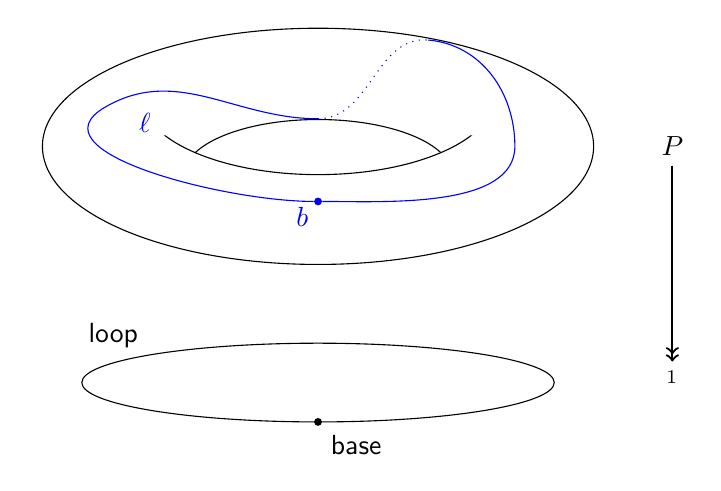
\begin{tikzpicture}
    \draw (0,0) ellipse (3 and .5);
    \draw (0,3) ellipse (3.5 and 1.5);
    \begin{scope}[yshift=4]
      \clip (-3,3) -- (-1.8,3) -- (-1.8,3.7) -- (1.8,3.7) -- (1.8,3) -- (3,3) -- (3,0) -- (-3,0) -- cycle;
      \draw[clip] (0,3.5) ellipse (2.25 and 1);
      \draw (0,2.5) ellipse (1.7 and .7);
    \end{scope}
    \node (P) at (4.5,3) {$P$};
    \node (S1) at (4.5,0) {$\Sn^1$};
    \draw[->>,thick] (P) -- (S1);
    \node[fill,circle,inner sep=1pt,label={below right:$\base$}] at (0,-.5) {};
    \node at (-2.6,.6) {$\lloop$};
    \node[fill,circle,blue,inner sep=1pt] (b) at (0,2.3) {};
    \node[blue] at (-.2,2.1) {$b$};
      \begin{scope}
        \draw[blue] (b) to[out=180,in=-150] (-2.7,3.5) to[out=30,in=180] (0,3.35);
        \draw[blue,dotted] (0,3.35) to[out=0,in=175] (1.4,4.35);
        \draw[blue] (1.4,4.35) to[out=-5,in=90] (2.5,3) to[out=-90,in=0,looseness=.8] (b);
      \end{scope}
      \node[blue] at (-2.2, 3.3) {$\ell$};
  \end{tikzpicture}
  \caption{The topological induction principle for $\Sn^1$}
  \label{fig:topS1ind}
\end{figure}

\begin{figure}
  \centering
  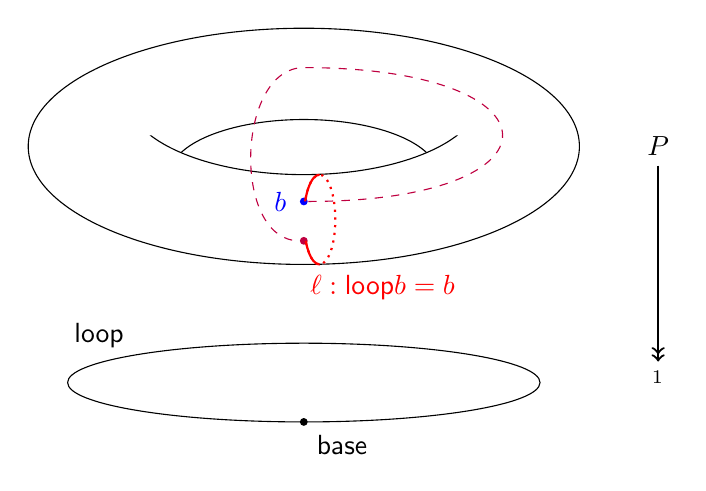
\begin{tikzpicture}
    \draw (0,0) ellipse (3 and .5);
    \draw (0,3) ellipse (3.5 and 1.5);
    \begin{scope}[yshift=4]
      \clip (-3,3) -- (-1.8,3) -- (-1.8,3.7) -- (1.8,3.7) -- (1.8,3) -- (3,3) -- (3,0) -- (-3,0) -- cycle;
      \draw[clip] (0,3.5) ellipse (2.25 and 1);
      \draw (0,2.5) ellipse (1.7 and .7);
    \end{scope}
    \node (P) at (4.5,3) {$P$};
    \node (S1) at (4.5,0) {$\Sn^1$};
    \draw[->>,thick] (P) -- (S1);
    \node[fill,circle,inner sep=1pt,label={below right:$\base$}] at (0,-.5) {};
    \node at (-2.6,.6) {$\lloop$};
    \node[fill,circle,blue,inner sep=1pt] (b) at (0,2.3) {};
      \node[blue] at (-.3,2.3) {$b$};
      \node[fill,circle,purple,inner sep=1pt] (tb) at (0,1.8) {};
      \draw[purple,dashed] (b) to[out=0,in=0,looseness=5] (0,4) to[out=180,in=180] (tb);
      \begin{scope}
        \clip (b) -- ++(.1,0) -- (.1,1.8) -- ++(-.2,0) -- ++(0,-1) -- ++(3,2) -- ++(-3,0) -- (-.1,2.3) -- cycle;
        \draw[red,dotted,thick] (.2,2.07) ellipse (.2 and .57);
        \begin{scope}
          % \draw[clip] (b) -- ++(.1,0) |- (tb) -- ++(-.2,0) -- ++(0,-1) -| ++(3,3) -| (b);
          \clip (.2,0) rectangle (-2,3);
          \draw[red,thick] (.2,2.07) ellipse (.2 and .57);
        \end{scope}
      \end{scope}
      \node[red] at (1,1.2) {$\ell: \trans \lloop b=b$};
  \end{tikzpicture}
  \caption{The type-theoretic induction principle for $\Sn^1$}
  \label{fig:ttS1ind}
\end{figure}

Of course, we expect to be able to prove the non-dependent elimination rule from the dependent one, by taking $P$ to be a constant type family.
This is in fact the case, although deriving the non-dependent computation rule for $\lloop$ (which refers to $\apfunc f$) from the dependent one (which refers to $\apdfunc f$) is surprisingly a little tricky.

\begin{lem}
  If $A$ is a type together with $x:A$ and $p:\id[A]xx$, then there is a
  function $f:\Sn^1\to{}A$ with
  \begin{align*}
    f(\base)&\jdeq x \\
    \apfunc f(\lloop)&=p
  \end{align*}
\end{lem}
\begin{proof}
  The two types $x=^{\lambda{}x.A}_\lloop{}x$ and $x=_Ax$ are not the same, but as we remarked in Chapter~\ref{cha:basics}, they are equivalent.
  Thus, from $p:x=x$ we can obtain $p':x=^{\lambda{}x.A}_\lloop{}x$, and thereby apply the induction principle to obtain $f:\Sn^1\to A$ such that $f(\base)\jdeq x$ and $\apdfunc f(\lloop) = p'$.
  It remains to derive the equality $\apfunc f(\lloop)=p$\dots
\end{proof}

Similarly, in this case we may speak of defining $f$ by $f(\base)\defeq x$ and $\ap f \lloop \defeq p$.
We also have an $\eta$-rule.

\begin{lem}
  If $A$ is a type and $f,g:\Sn^1\to{}A$ are two maps together with two
  equalities $p,q$:
  \begin{align*}
    p:f(\base)&=_Ag(\base)\\
    q:\map{f}\lloop&=^{\lambda{}x.\,x=_Ax}_p\map{g}\lloop
  \end{align*}
  Then for all $x:\Sn^1$ we have $f(x)=g(x)$.
\end{lem}
\begin{proof}
  This is the dependent elimination rule for the type family $P(x)\defeq(f(x)=g(x))$.
\end{proof}

These two lemmas imply the expected universal property of the circle:

\begin{lem}
  For any type $A$ we have a natural equivalence
  \[ (\Sn^1 \to A) \;\simeq\;
  \sm{x:A} (x=x).
  \]
\end{lem}
\begin{proof}
  We have a canonical function $f:(\Sn^1 \to A) \to \sm{x:A} (x=x)$ defined by $f(g) \defeq (g(\base),\ap g \lloop)$.
  The non-dependent eliminator shows that the fibers of $f$ are inhabited, while the $\eta$-rule shows that they are mere propositions.
  Hence they are contractible, so $f$ is an equivalence.
\end{proof}

For other higher inductive types, we will generally leave the proofs of these lemmas to the reader.
We now proceed to consider many examples.


\section{The interval}
\label{sec:interval}

The \emph{interval} $I$ is perhaps an even simpler higher inductive type than the circle.
It is generated by:
\begin{itemize}
\item a point $0:I$,
\item a point $1:I$, and
\item a path $\seg : \id[I]01$.
\end{itemize}
The recursion principle for the interval says that given a type $B$ along with
\begin{itemize}
\item a point $b_0:B$,
\item a point $b_1:B$, and
\item a path $s:b_0=b_1$,
\end{itemize}
there is a function $f:I\to B$ such that $f(0)\jdeq b_0$, $f(1)\jdeq b_1$, and $\ap f \seg = s$.
The induction principle says that given $P:I\to\type$ along with
\begin{itemize}
\item a point $b_0:P(0)$,
\item a point $b_1:P(1)$, and
\item a path $s:\dpath{P}{\seg}{b_0}{b_1}$,
\end{itemize}
there is a function $f:\prd{x:I} P(x)$ such that $f(0)\jdeq b_0$, $f(1)\jdeq b_1$, and $\apd f \seg = s$.

From the point of view of homotopy theory, of course, the interval is not really interesting:

\begin{lem}
  The type $I$ is contractible.
\end{lem}

\begin{proof}
  We will prove that for all $x:I$ we have $x=_I1$. In other words we want a
  function $f$ of type $\prd{x:I}(x=_I1)$. We begin to define $f$ in the following way:
  \begin{alignat*}{2}
    f(0)&\defeq \seg  &:0&=_I1\\
    f(1)&\defeq \refl1 &:1 &=_I1
  \end{alignat*}
  It remains to define $\apd{f}\seg$, which must have type $\seg =_\seg^{\lambda{}x.x=_I1}\refl 1$.
  By definition this type is $\trans\seg\seg=_{1=_I1}\refl1$, which in turn is equivalent to $\rev\seg\ct\seg=\refl1$.
  But there is a canonical term of that type, namely the proof that path inverses are in fact inverses.
\end{proof}

However, type-theoretically the interval is not completely boring, because it enables us to give an easy proof of function extensionality.

\begin{lem}
  If $f,g:A\to{}B$ are two functions such that $f(x)=g(x)$ for every $x:A$, then
  $f=g$ in the type $A\to{}B$.
\end{lem}

\begin{proof}
  Let's call the proof we have $p:\prd{x:A}(f(x)=g(x))$. For all $x:A$ we define
  a function $\widetilde{p}_x:I\to{}B$ by
  \begin{align*}
    \widetilde{p}_x(0) &= f(x) \\
    \widetilde{p}_x(1) &= g(x) \\
    \map{(\widetilde{p}_x)}\seg &= p(x)
  \end{align*}
  We now define $q:I\to(A\to{}B)$ by
  \[q(i)\defeq(\lambda{}x.\,\widetilde{p}_x(i))\]
  Then $q(0)$ is the function $\lambda{}x.\,\widetilde{p}_x(0)$, which is equal to $f$ because $\widetilde{p}_x(0)$ is defined by $f(x)$.
  Similarly, we have $q(1)=g$, and hence
  \[\map{q}\seg:f=_{(A\to{}B)}g \qedhere\]
\end{proof}

\section{Circles and spheres}
\label{sec:circle}

\section{Suspensions}
\label{sec:suspension}

\section{Cell complexes}
\label{sec:cell-complexes}

\section{Pushouts}
\label{sec:colimits}

TODO: move section on pushouts as HITs from the next chapter.

\section{Quotients}
\label{sec:quotients}

Both as HIT and impredicatively.

\section{Truncations}
\label{sec:truncations}

\section{Free algebras}
\label{sec:free-algebras}

\section{The flattening lemma}
\label{sec:flattening}

The flattening lemma is a general lemma about higher inductive types which says
that if $W$ is a higher inductive type and $P:W\to\type$ is a function defined
by induction and with the univalence axiom for the paths, then the total space
of $P$ is equivalent to a ``flattened'' higher inductive type build up from $W$
and $P$.

In what follows, we will assume that we have $A,B:\type$ and $f,g:B\to{}A$ and
that the higher inductive type $W$ is of the form

\newcommand{\cc}{\mathsf{c}}
\newcommand{\pp}{\mathsf{p}}
\newcommand{\cct}{\widetilde{\mathsf{c}}}
\newcommand{\ppt}{\widetilde{\mathsf{p}}}

\begin{align*}
  W \defeq&\ |\ \cc:A\to{}W\\
  &\ |\ \pp:\prd{b:B}\cc(f(b))=_W\cc(g(b))
\end{align*}

Using binary sums and dependent sums a lot of interesting nonrecursive higher
inductive types can be represented in this form. All point constructors have to
be bundled in the type $A$ and all path constructors in the type $B$.

\begin{lem}[Flattening lemma]
  If $C:A\to\type$ is a family of types over $A$ and
  $D:\prd{b:B}C(f(b))\simeq{}C(g(b))$ is a family of equivalences over $B$, we
  can define a function
  \begin{align*}
    P &: W\to\type\\
    P(\cc(a)) &= C(a)\\
    \map{P}{\pp(b)} &= \eqtopath(D(b))
  \end{align*}

  We define another higher inductive type:
  \begin{align*}
    \widetilde{W} \defeq&\ |\ \cct:\prd{a:A}{x:C(a)}\widetilde{W}\\
    &\ |\
    \ppt:\prd{b:B}{x:C(f(b))}\cct(f(b),x)=_{\widetilde{W}}\cct(g(b),D(b)(x))
  \end{align*}

  The statement of the flattening lemma is that the total space of $P$ is
  equivalent to $\widetilde{W}$.
\end{lem}

\begin{proof}
  We will define two maps going back and forth and prove that they are inverse
  to each other.

  The map $f:\widetilde{W}\to\Sigma_{x:W}P(x)$ is defined by
  \begin{align*}
    f(\cct(a,x)) &= (\cc(a),x) \\
    \map{f}{\ppt(b,y)} &= (\pp(b),\map{(\lambda{}f.\,f\,x)}{\eqtopath(D(b))}
  \end{align*}

  For the inverse map $g:\Sigma_{x:W}P(x)\to\widetilde{W}$ we currify and define
  for all $x:W$ a map $\widetilde{g}_x:P(x)\to\widetilde{W}$ by induction on
  $x$.

  \emph{unfinished}
  % \begin{align*}
  %   \widetilde{g}_{\cc(a)} &= \lambda{}x^{C(a)}.\,\cct(a,x) \\
  %   \map{(\lambda{}x^W.\,\widetilde{g}_x)}{\pp(b)} &= 
  % \end{align*}
\end{proof}


% Local Variables:
% TeX-master: "main"
% End:
